
\section{Tafel ronde 1: Slimste mens}
Freddy doet mee met de slimste mens, help jij hem?
geef de naam van de persoon waarop freddy is geplakt

\begin{questions}

\question[2] {
\begin{center}
{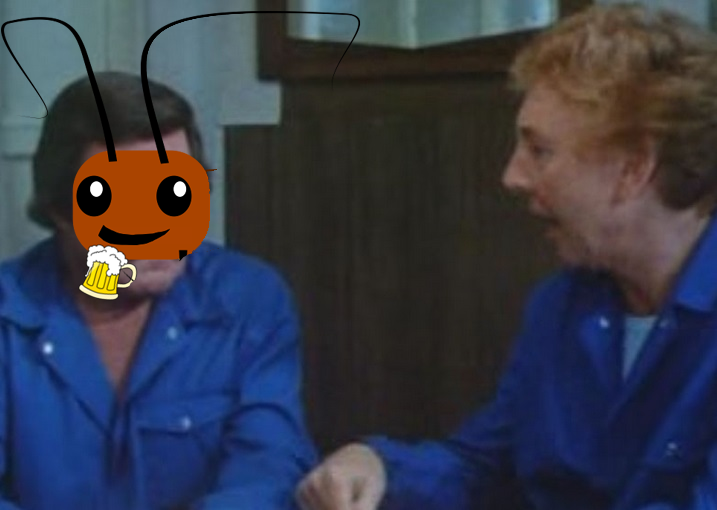
\includegraphics[scale=0.40]{1}}
\end{center}
\begin{flushleft}
\makebox[\textwidth]{Volledige naam:\enspace\hrulefill}
\end{flushleft} }
\question[2] {
\begin{center}
{
\includegraphics[scale=0.20]{2}}
\end{center}
\begin{flushleft}
\makebox[\textwidth]{naam:\enspace\hrulefill}
\end{flushleft} }
\question[1] {
\begin{center}
{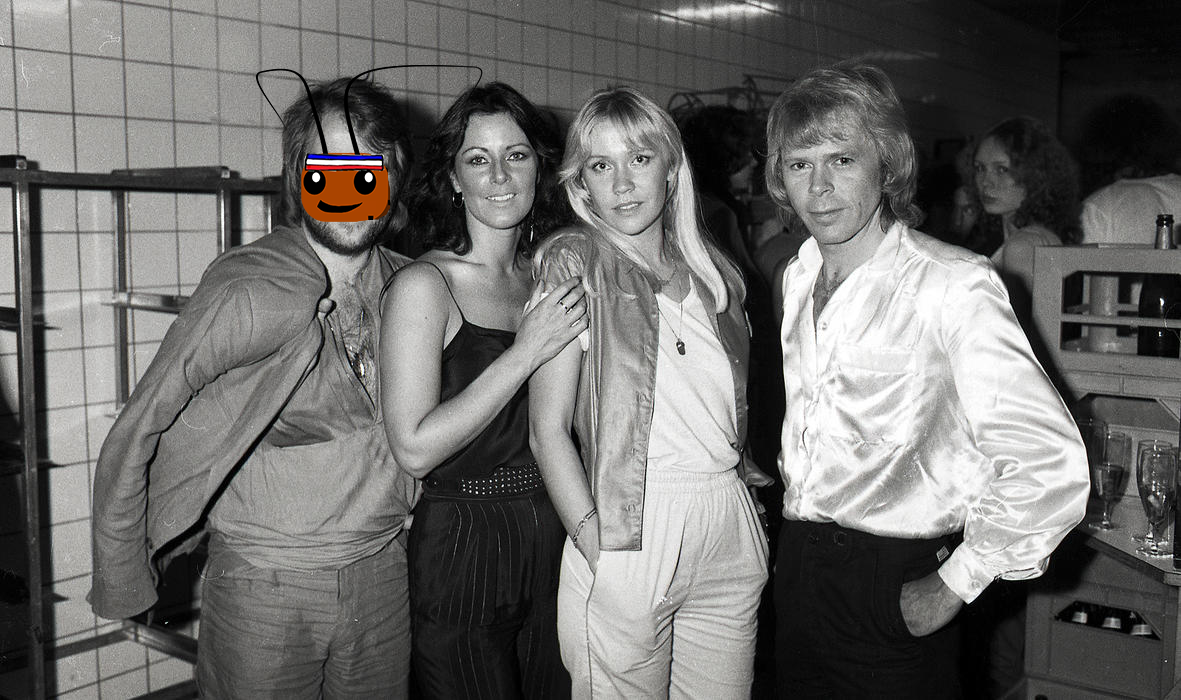
\includegraphics[scale=0.30]{3}}
\end{center}
\begin{flushleft}
\makebox[\textwidth]{naam:\enspace\hrulefill}
\end{flushleft} }
\question[1] {
\begin{center}
{
\includegraphics[scale=0.15]{4}}
\end{center}
\begin{flushleft}
\makebox[\textwidth]{naam:\enspace\hrulefill}
\end{flushleft} }
\question[1] {
\begin{center}
{
\includegraphics[scale=0.80]{5}}
\end{center}
\begin{flushleft}
\makebox[\textwidth]{naam:\enspace\hrulefill}
\end{flushleft} }

\question[3]{
{
\begin{table}[h]
\centering
\begin{tabular}{llll}
\textbf{Amerikaan} & \textbf{1949}          & \textbf{dokter Mabuse} & \textbf{911}    \\
\textbf{1813}      & \textbf{7 gele truien} & \textbf{Protest}       & \textbf{1722}   \\
\textbf{Studenten} & \textbf{112}           & \textbf{Gent}          & \textbf{kanker}
\end{tabular}
\end{table}
}
\begin{flushleft}
\makebox[\textwidth]{Link 1:\enspace\hrulefill\linebreak}
\makebox[\textwidth]{Link 2:\enspace\hrulefill}
\makebox[\textwidth]{Link 3:\enspace\hrulefill}
\end{flushleft}
}

\question[3]{
{\begin{table}[h]
\centering
\begin{tabular}{llll}
\textbf{Schuilhuis} & \textbf{November 1938}          & \textbf{Onderduiken} & \textbf{Aanval tegen joden}    \\
\textbf{verbranden}      & \textbf{joods meisje} & \textbf{Pogroms}       & \textbf{nummer}   \\
\textbf{glaswerk} & \textbf{Joden}           & \textbf{dagboek}          & \textbf{Auschwitz}
\end{tabular}
\end{table}
}
\begin{flushleft}
\makebox[\textwidth]{Link 1:\enspace\hrulefill}
\makebox[\textwidth]{Link 2:\enspace\hrulefill}
\makebox[\textwidth]{Link 3:\enspace\hrulefill}
\end{flushleft}
}

\question[3]{
{\begin{table}[h]
\centering
\begin{tabular}{llll}
\textbf{CSI} & \textbf{Brusel}          & \textbf{sunrise} & \textbf{London}    \\
\textbf{De kotmadam}      & \textbf{Temptation island} & \textbf{zout}       & \textbf{The Simpsons}   \\
\textbf{Parijs} & \textbf{Mexicaans}           & \textbf{Amsterdam}          & \textbf{citroen}
\end{tabular}
\end{table}
}
\begin{flushleft}
\makebox[\textwidth]{Link 1:\enspace\hrulefill}
\makebox[\textwidth]{Link 2:\enspace\hrulefill}
\makebox[\textwidth]{Link 3:\enspace\hrulefill}
\end{flushleft}
}
\newpage
\question[3]{
{\begin{table}[h]
\centering
\begin{tabular}{llll}
\textbf{Pessarium} & \textbf{klein}          & \textbf{buitenaars} & \textbf{nek}    \\
\textbf{letsel}      & \textbf{telefoneren} & \textbf{spiraaltje}       & \textbf{zweepslag}   \\
\textbf{Spielberg} & \textbf{De pil}           & \textbf{Van voor naar achter}          & \textbf{condoom}
\end{tabular}
\end{table}
}
\begin{flushleft}
\makebox[\textwidth]{Link 1:\enspace\hrulefill}
\makebox[\textwidth]{Link 2:\enspace\hrulefill}
\makebox[\textwidth]{Link 3:\enspace\hrulefill}
\end{flushleft}
}
\question[3]{
{\begin{table}[h]
\centering
\begin{tabular}{llll}
\textbf{Neuswrat} & \textbf{rapper}          & \textbf{brandstapel} & \textbf{papier}    \\
\textbf{Amerikaan}      & \textbf{Kraanvogel} & \textbf{bezem}       & \textbf{genie in Alladin}   \\
\textbf{vouwen} & \textbf{vrouw}           & \textbf{Acteur}          & \textbf{Japans}
\end{tabular}
\end{table}
}
\begin{flushleft}
\makebox[\textwidth]{Link 1:\enspace\hrulefill}
\makebox[\textwidth]{Link 2:\enspace\hrulefill}
\makebox[\textwidth]{Link 3:\enspace\hrulefill}
\end{flushleft}
}

\end{questions}

\begin{table}[!b]
\centering
\begin{tabular}{|l|l|l|l|l|l|l|l|l|l|l|l}
\hline
Vraag       & 1 & 2 & 3 & 4 & 5 & 6 & 7 & 8 & 9 & 10 \\ \hline
max. punten & 1 & 1 & 1 & 1 & 1 & 3 & 3 & 3 & 3 & 3\\ \hline
score       &   &   &   &   &   &   &   &   &   &  \\ \hline
\end{tabular}
\end{table}
\newpage